\documentclass[12pt]{article}
\usepackage[utf8]{inputenc}
\usepackage{amsmath, amssymb, amsthm}
\usepackage{enumitem}
\usepackage{geometry}
\usepackage{fancyhdr}
\usepackage{pgfplots}
\usepackage{tikz}
\usepackage{float}
\usepackage{graphicx}
\DeclareMathOperator{\Tr}{Tr}
\DeclareMathOperator{\rng}{rng}
\DeclareMathOperator{\norm}{||}
\DeclareMathOperator{\NN}{\mathbb{N}}
\DeclareMathOperator{\ZZ}{\mathbb{Z}}
\DeclareMathOperator{\QQ}{\mathbb{Q}}
\DeclareMathOperator{\RR}{\mathbb{R}}
\DeclareMathOperator{\CC}{\mathbb{C}}

% Page setup
\setlength{\headheight}{15pt}
\geometry{letterpaper, margin=1in}
\setlength{\parindent}{0pt}
\setlength{\parskip}{1em}
\pagestyle{fancy}
\fancyhf{}
\fancyhead[L]{\textbf{Sebastian Griego}}  % Replace with your name
\fancyhead[C]{\textbf{ODEs}}  % Replace with your course name
\fancyhead[R]{\textbf{Midterm 1}}  % Replace with your assignment number
\fancyfoot[C]{\thepage}

\newenvironment{problem}[1]{
    \textbf{Problem #1:}
}{
    \rmfamily \vspace{2em}
}

\newenvironment{solution}{
    \textbf{Solution:}
    
}{
    
    \vspace{2em}
}

\begin{document}

\title{Midterm 1}  % Replace with the homework number
\author{Sebastian Griego}  % Replace with your name
\maketitle

\begin{problem}{1}
    For all \(t \geq 0\), solve the differential equation
    \[
        \frac{dy}{dt} + y = f(t), \quad y(0) = y_0
    \]
    where \(f(t)\) is periodic with period \(T \), i.e. \(f(t+T) = f(t)\), and on \([0,T]\), \(f(t)\) is defined to be
    \[
        f(t) = \begin{cases} 
            1 & 0 \leq t < \frac{T}{2} \\
            0 & \frac{T}{2} \leq t < T
        \end{cases}
    \]
\end{problem}

\begin{solution}
    Define the integrating factor,
    \[
        \Phi(t, s) = e^{-\int_s^t 1 dt} = e^{s-t}
    \]
    Solution to the ODE:
    \[
        \begin{aligned}
            y(t) &= \Phi(t, 0) \cdot y(0) + \int_0^t \Phi(t, s) \cdot f(s) ds \\
            &= e^{-t} \cdot y_0 + \int_0^t e^{s-t} \cdot f(s) ds \\
        \end{aligned}
    \]
    Evaluate the integral for each interval of \(f(t)\):
    \begin{itemize}
        \item For \(0 \leq t < \frac{T}{2}\):
        \[
            \int_0^t e^{s-t} \cdot 1 ds = \int_0^t e^{s-t} ds = e^{s-t} \bigg|_{0}^{t} = e^{t-t} - e^{0-t} = 1 - e^{-t}
        \]
        \item For \(\frac{T}{2} \leq t < T\):
        \[
            \int_0^\frac{T}{2} e^{s-t} \cdot 1 ds + \int_\frac{T}{2}^t e^{s-t} \cdot 0 ds = \int_0^\frac{T}{2} e^{s-t} ds = e^{s-t} \bigg|_{0}^{\frac{T}{2}} = e^{\frac{T}{2}-t} - e^{-t}
        \]
        \item For \(T \leq t < \frac{3T}{2}\):
        \[
            \begin{aligned}
                \int_0^\frac{T}{2} e^{s-t} \cdot 1 ds + \int_\frac{T}{2}^T e^{s-t} \cdot 0 ds + \int_T^t e^{s-t} \cdot 1 ds &= \int_0^\frac{T}{2} e^{s-t} ds + \int_T^t e^{s-t} ds \\
                &= e^{\frac{T}{2}-t} - e^{-t} + e^{t-t} - e^{T-t} \\
                &= e^{\frac{T}{2}-t} - e^{-t} + 1 - e^{T-t}
            \end{aligned}
        \]
        \item For \(\frac{3T}{2} \leq t < 2T\):
        \[
            \begin{aligned}
                \int_0^\frac{T}{2} e^{s-t} \cdot 1 ds + 0 + \int_{T}^\frac{3T}{2} e^{s-t} \cdot 1 ds + 0  &= \int_0^\frac{T}{2} e^{s-t} ds + \int_{T}^\frac{3T}{2} e^{s-t} ds \\
                &= (e^{\frac{T}{2}-t} - e^{-t}) + (e^{\frac{3T}{2}-t} - e^{T-t}) \\
            \end{aligned}
        \]
    \end{itemize}
    Note:
    \[
        \int_0^T = \int_{0}^{\frac{T}{2}}
    \]
    There is a pattern:
    \[
        \begin{aligned}
            \int_0^T e^{s-t} ds &= e^{\frac{T}{2}-t} - e^{-t} \\
            \int_{T}^{2T} e^{s-t} ds &= e^{\frac{3T}{2}-t} - e^{T-t}
        \end{aligned}
    \]
    Generalizing,
    \[
        \int_{kT}^{(k+1)T} e^{s-t} ds = e^{\frac{(2k+1)T}{2}-t} - e^{kT-t}
    \]
    Therefore,
    \[
        \int_0^t e^{s-t} ds = \sum_{j=0}^{n - 1} \int_{jT}^{(j+1)T} e^{s-t} ds + \int_{nT}^t e^{s-t} ds
    \]
    The solution is
    \[
        \begin{aligned}
            y(t) &= e^{-t}y_0 + \sum_{j=0}^{n-1} \int_{jT}^{(j+1)T} e^{s-t} ds + \int_{nT}^t e^{s-t} ds \\
            &= e^{-t}y_0 + \sum_{j=0}^{n-1} (e^{\frac{(2j+1)T}{2}-t} - e^{jT-t}) + \int_{nT}^t e^{s-t} ds\\
            &= e^{-t}y_0 + \sum_{j=0}^{n-1} (e^{jT} \cdot e^{\frac{T}{2}-t} - e^{jT} \cdot e^{-t}) + \int_{nT}^t e^{s-t} ds \\
            &= e^{-t}y_0 + \sum_{j=0}^{n-1} e^{jT} (e^{\frac{T}{2}-t} - e^{-t}) + \int_{nT}^t e^{s-t} ds \\
            &= e^{-t}y_0 + (e^{\frac{T}{2}-t} - e^{-t}) \sum_{j=0}^{n-1} e^{jT} + \int_{nT}^t e^{s-t} ds \\
        \end{aligned}
    \]
    Consider the identity
    \[
        \sum_{j=0}^{n-1} e^{jT} = \frac{e^{nT} - 1}{e^T - 1}
    \]
    Therefore,
    \[
        \begin{aligned}
            y(t) &= e^{-t}y_0 + (e^{\frac{T}{2}-t} - e^{-t}) \cdot \frac{e^{nT} - 1}{e^T - 1} + \int_{nT}^t e^{s-t} ds \\
            &= e^{-t}y_0 + (e^{\frac{T}{2}-t} - e^{-t}) \cdot \frac{e^{nT} - 1}{e^T - 1} + (1 - e^{nT-t})
        \end{aligned}
    \]
    where \(n = \lfloor \frac{t}{T} \rfloor\).
    
\end{solution}

\newpage

\begin{problem}{2}
    Sketch the phase portraits corresponding to the matrices
    \[
        A = \begin{pmatrix}
            1 & 3 \\
            3 & 1
        \end{pmatrix}, \quad
        A = \begin{pmatrix}
            3 & -2 \\
            5 & -2
        \end{pmatrix}, \quad
        A = \begin{pmatrix}
            -1 & 1 \\
            1 & -1
        \end{pmatrix}
    \]
\end{problem}

\begin{solution}
    For,
    \[
        A = \begin{pmatrix}
            1 & 3 \\
            3 & 1
        \end{pmatrix}
    \]
    Find the eigenvalues,
    \[
        \begin{aligned}
            \lambda &= \frac{1}{2}(\Tr(A) \pm \sqrt{\Tr(A)^2 - 4 \det(A)}) \\
            &= \frac{1}{2}(2 \pm \sqrt{4 - 4(-8)}) \\
            &= \frac{1}{2}(2 \pm \sqrt{36}) \\
            &= \frac{1}{2}(2 \pm 6) \\
            &= 1 \pm 3 \\
            &= -2, 4
        \end{aligned}
    \]
    This is a saddle. Find the eigenvectors for \(\lambda = -2\),
    \[
        \begin{aligned}
            \begin{pmatrix}
                3 & 3 \\
                3 & 3
            \end{pmatrix} \begin{pmatrix} x_1 \\ x_2 \end{pmatrix} = \begin{pmatrix} 0 \\ 0 \end{pmatrix}\\
            3x_1 + 3x_2 &= 0 \\
            x_1 &= -x_2
        \end{aligned}
    \]
    So the eigenvector for \(\lambda = -2\) is \(\begin{pmatrix} 1 \\ -1 \end{pmatrix}\). \(\lambda < 0 \), so this goes towards the origin.

    Find the eigenvectors for \(\lambda = 4\),
    \[
        \begin{aligned}
            \begin{pmatrix}
                -3 & 3 \\
                3 & -3
            \end{pmatrix} \begin{pmatrix} x_1 \\ x_2 \end{pmatrix} = \begin{pmatrix} 0 \\ 0 \end{pmatrix} \\
            -3x_1 + 3x_2 &= 0 \\
            x_1 &= x_2
        \end{aligned}
    \]
    So the eigenvector for \(\lambda = 4\) is \(\begin{pmatrix} 1 \\ 1 \end{pmatrix}\). \(\lambda > 0 \), so this goes away from the origin.


    For,
    \[
        A = \begin{pmatrix}
            3 & -2 \\
            5 & -2
        \end{pmatrix}
    \]
    Find the eigenvalues,
    \[
        \begin{aligned}
            \lambda &= \frac{1}{2}(1 \pm \sqrt{ 1^2 - 4 \cdot 4}) \\
            &= \frac{1}{2}(1 \pm \sqrt{-15}) \\
            &= \frac{1}{2}(1 \pm i \sqrt{15})
        \end{aligned}
    \]
    \(\lambda \in \CC\), so this is a spiral. \(\Tr(A) > 0\) and \(\det(A) > 0\), so this spirals outwards from the origin.


    For,
    \[
        A = \begin{pmatrix}
            -1 & 1 \\
            1 & -1
        \end{pmatrix}
    \]
    Find the eigenvalues,
    \[
        \begin{aligned}
            \lambda &= \frac{1}{2}(-2 \pm \sqrt{(-2)^2 - 4 \cdot 0})\\
            &= \frac{1}{2}(-2 \pm 2) \\
            &= -2, 0
        \end{aligned}
    \]
    Find the eigenvectors for \(\lambda = -2\),
    \[
        \begin{aligned}
            \begin{pmatrix}
                1 & 1 \\
                1 & 1
            \end{pmatrix} \begin{pmatrix} x_1 \\ x_2 \end{pmatrix} = \begin{pmatrix} 0 \\ 0 \end{pmatrix} \\
            x_1 + x_2 &= 0 \\
            x_1 &= -x_2
        \end{aligned}
    \]
    So the eigenvector for \(\lambda = -2\) is \(\begin{pmatrix} 1 \\ -1 \end{pmatrix}\). \(\lambda < 0 \), so this goes towards the origin.

    Find the eigenvectors for \(\lambda = 0\),
    \[
        \begin{aligned}
            \begin{pmatrix}
                -1 & 1 \\
                1 & -1
            \end{pmatrix} \begin{pmatrix} x_1 \\ x_2 \end{pmatrix} = \begin{pmatrix} 0 \\ 0 \end{pmatrix} \\
            -x_1 + x_2 &= 0 \\
            x_1 &= x_2
        \end{aligned}
    \]
    So the eigenvector for \(\lambda = 0\) is \(\begin{pmatrix} 1 \\ 1 \end{pmatrix}\). \(\lambda = 0 \), so this nothing moves on this vector.

    Phase planes:
    \begin{figure}[H]
        \centering
        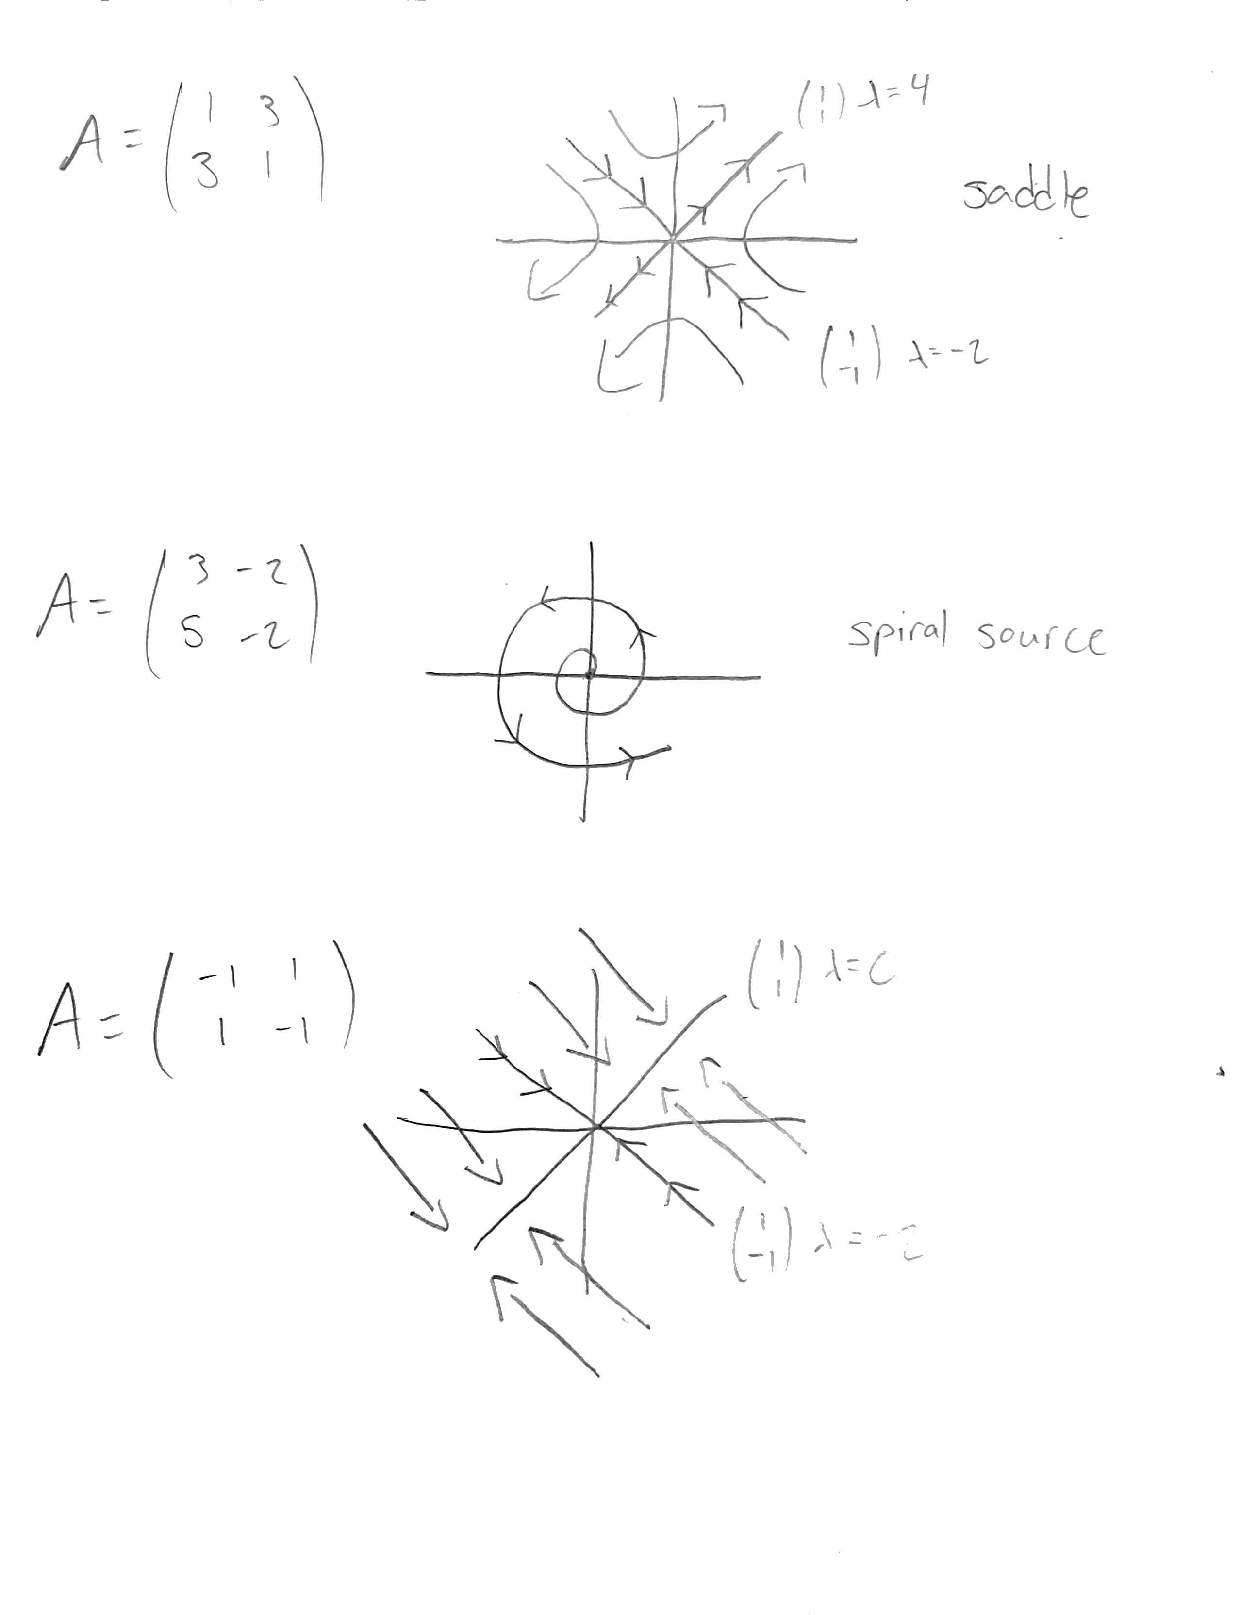
\includegraphics[width=0.8\textwidth]{Mid_phase.pdf}
        \caption{Phase planes}
    \end{figure}
    
\end{solution}

\newpage

\begin{problem}{3}
    Solve the differential equation
    \[
        \frac{d\vec{x}}{dt} = A\vec{x}, \; x(0) = x_0
    \]
    for,
    \[
        A = \begin{pmatrix}
            1 & 0 & 0 \\
            0 & 2 & 0 \\
            0 & 0 & 3
        \end{pmatrix}, \quad A = \begin{pmatrix}
            2 & 0 & 0 \\
            0 & 5 & -1 \\
            0 & 1 & 3
        \end{pmatrix}
    \]
\end{problem}

\begin{solution}
    For,
    \[
        A = \begin{pmatrix}
            1 & 0 & 0 \\
            0 & 2 & 0 \\
            0 & 0 & 3
        \end{pmatrix}
    \]
    The matrix is diagonal, so the eigenvalues are
    \[
        \lambda = 1, 2, 3
    \]
    and the eigenvectors are
    \[
        \begin{pmatrix} 1 \\ 0 \\ 0 \end{pmatrix}, \begin{pmatrix} 0 \\ 1 \\ 0 \end{pmatrix}, \begin{pmatrix} 0 \\ 0 \\ 1 \end{pmatrix}
    \]
    Both \(V\) and \(V^{-1}\) are the identity matrix, so the equation is
    \[
        \frac{d\vec{x}}{dt} = V \Lambda V^{-1} \vec{x} = \Lambda \vec{x}
    \]
    with general solution
    \[
        \vec{x}(t) = V \begin{pmatrix} e^{\lambda_1 t} & 0 & 0 \\ 0 & e^{\lambda_2 t} & 0 \\ 0 & 0 & e^{\lambda_3 t} \end{pmatrix} V^{-1} \vec{x_0} = I \begin{pmatrix} e^{\lambda_1 t} & 0 & 0 \\ 0 & e^{\lambda_2 t} & 0 \\ 0 & 0 & e^{\lambda_3 t} \end{pmatrix} I \vec{x_0}
    \]
    The solution is
    \[
        \vec{x}(t) = \begin{pmatrix} e^t & 0 & 0 \\ 0 & e^{2t} & 0 \\ 0 & 0 & e^{3t} \end{pmatrix} \vec{x_0}
    \]
    Now, for 
    \[
        A = \begin{pmatrix}
            2 & 0 & 0 \\
            0 & 5 & -1 \\
            0 & 1 & 3
        \end{pmatrix}
    \]
    One eigenvalue is \(\lambda = 2\) with eigenvector \(\begin{pmatrix} 1 \\ 0 \\ 0 \end{pmatrix}\).

    Now look at the \(2 \times 2\) matrix,
    \[
        \begin{pmatrix}
            5 & -1 \\
            1 & 3
        \end{pmatrix}
    \]
    Find the eigenvalues,
    \[
        \begin{aligned}
            \lambda &= \frac{1}{2}(8 \pm \sqrt{64 - 64}) \\
            &= 4
        \end{aligned}
    \]
    This is a repeated eigenvalue. Find the eigenvectors for \(\lambda = 4\),
    \[
        \begin{pmatrix}
            1 & -1 \\
            1 & -1
        \end{pmatrix} \begin{pmatrix} x_1 \\ x_2 \end{pmatrix} = \begin{pmatrix} 0 \\ 0 \end{pmatrix}
    \]
    The eigenvector is \(\begin{pmatrix} 1 \\ 1 \end{pmatrix}\) for the \(2 \times 2\) matrix, and \(\begin{pmatrix} 0 \\ 1 \\ 1 \end{pmatrix}\) for the \(3 \times 3\) matrix.

    Find \(\vec{u}\) where \((A - 4I)\vec{u} = \vec{v}\)
    \[
        \begin{pmatrix}
            -2 & 0 & 0 \\
            0 & 1 & -1 \\
            0 & 1 & -1
        \end{pmatrix} \begin{pmatrix} x_1 \\ x_2 \\ x_3 \end{pmatrix} = \begin{pmatrix} 0 \\ 1 \\ 1 \end{pmatrix}
    \]
    \[
        x_2 - x_3 = 1
    \]
    So \(\vec{u} = \begin{pmatrix} 0 \\ 1 \\ 0 \end{pmatrix}\).

    The Jordan decomposition is
    \[
        A = \begin{pmatrix} 1 & 0 & 0 \\ 0 & 1 & 1 \\ 0 & 0 & 1 \end{pmatrix} \begin{pmatrix} 2 & 0 & 0 \\ 0 & 4 & 1 \\ 0 & 0 & 4 \end{pmatrix} \begin{pmatrix} 1 & 0 & 0 \\ 0 & 1 & 1 \\ 0 & 0 & 1 \end{pmatrix}^{-1}
    \]
    The solution is
    \[
        \begin{aligned}
            \vec{x}(t) &= V \begin{pmatrix} e^{\lambda_1 t} & 0 & 0 \\ 0 & e^{\lambda_2 t} & te^{\lambda_2 t} \\ 0 & 0 & e^{\lambda_2 t} \end{pmatrix} V^{-1} \vec{x_0}\\
            &= \begin{pmatrix} 1 & 0 & 0 \\ 0 & 1 & 1 \\ 0 & 0 & 1 \end{pmatrix} \begin{pmatrix} e^{2t} & 0 & 0 \\ 0 & e^{4t} & te^{4t} \\ 0 & 0 & e^{4t} \end{pmatrix} \begin{pmatrix} 1 & 0 & 0 \\ 0 & 0 & 1 \\ 0 & 1 & -1 \end{pmatrix} \vec{x_0}
        \end{aligned}
    \]
    

\end{solution}

\newpage

\begin{problem}{4}
    Assuming \(||A|| < 1\) and using
    \[
        (I - A)^{-1} = \sum_{j=0}^{\infty} A^j
    \]
    prove the inequalities,
    \[
        ||(I - A)^{-1}|| \leq \frac{||A||}{1 - ||A||}
    \]
    and
    \[
        \left|\left|\sum_{j=m}^{\infty} \frac{1}{j!}A^j \right|\right| \leq \frac{||A||^m}{m!}\frac{1}{1 - ||A||}
    \]
\end{problem}

\begin{solution}
    \begin{proof}
        \[
        \begin{aligned}
            ||(I - A)^{-1} - I||&= \left|\left|\sum_{j=0}^{\infty} A^j - I \right|\right| \\
            &= \left|\left|\sum_{j=1}^{\infty} A^j \right|\right| \\
            &\leq \sum_{j=1}^{\infty} ||A^j|| \\
            &\leq \sum_{j=1}^{\infty} ||A||^j \\
            &= \frac{||A||}{1 - ||A||} \quad \text{because it's a geometric series and } ||A|| < 1
        \end{aligned}
    \]
    Therefore,
    \[
        ||(I - A)^{-1} - I|| \leq \frac{||A||}{1 - ||A||}
    \]
    \end{proof}
    Now the other inequality where \(j > m\),
    \begin{proof}
        \[
            \begin{aligned}
                \left|\left|\sum_{j=m}^{\infty} \frac{1}{j!}A^j \right|\right| &\leq \sum_{j=m}^{\infty} \frac{1}{j!} ||A^j|| \\
                &\leq \sum_{j=m}^{\infty} \frac{1}{j!} ||A||^j \\
                &= \frac{||A||^m}{m!} + \frac{||A||^{m+1}}{(m+1)!} + \frac{||A||^{m+2}}{(m+2)!} + \cdots \\
                &= \frac{||A||^m}{m!} \left(1 + \frac{||A||}{m+1} + \frac{||A||^2}{(m+1)(m+2)} + \cdots \right) \\
                &\leq \frac{||A||^m}{m!} (1 + ||A|| + ||A||^2 + \cdots) \\
                &= \frac{||A||^m}{m!} \sum_{j=0}^{\infty} ||A||^j \\
                &= \frac{||A||^m}{m!} \frac{1}{1 - ||A||}
            \end{aligned}
        \]
    Therefore,
    \[
        \left|\left|\sum_{j=m}^{\infty} \frac{1}{j!}A^j \right|\right| \leq \frac{||A||^m}{m!}\frac{1}{1 - ||A||}
    \]
    \end{proof}
\end{solution}

\newpage

\begin{problem}{5}
    For \(A\) a real \(2 \times 2\) matrix and \(\vec{x} \in \RR^2\) and \(\vec{f}(T) \in \RR^2\), with each entry \(f_j(t)\) assumed to be continuous
    \begin{itemize}
        \item Show that the solution to the initial value problem
        \[
            \frac{d\vec{x}}{dt} = A\vec{x} + \vec{f}(t), \; \vec{x}(0) = \vec{x}_0
        \]
        is given by
        \[
            \vec{x}(t) = e^{At}\vec{x}_0 + e^{At} \int_0^t e^{-As} \vec{f}(s) ds
        \]
        \item Now let \(A\) be such that \(A^T = -A\). Show that
        \[
            A = \begin{pmatrix} 0 & \omega \\ -\omega & 0 \end{pmatrix}
        \]
        for some real value \(\omega\). Now suppose the forcing \(\vec{f}(t)\) is such that
        \[
            \vec{f}_j(t) = \cos(\lambda_j t), \; \lambda_j  \in \RR, \; j = 1, 2
        \]
        Show by direct computation that if either \(\lambda_1 = \omega\) or \(\lambda_2 = \omega\), then you get terms in your solution \(\vec{x}(t)\) which grow linearly, and thus
        unboundedly, in \(t\).
    \end{itemize}
\end{problem}

\begin{solution}
    \textbf{Part 1}
    
    Define:
    \[
        \begin{aligned}
            \Phi(t) &= e^{-At}\\
            \vec{z}(t) &= \Phi(t)\vec{x}
        \end{aligned}
    \]
    Then,    
    \[
        \begin{aligned}
            \frac{d}{dt}\vec{z}(t) &= \frac{d}{dt}\left(\Phi(t)\vec{x}\right) \\
            &= \frac{d\Phi(t)}{dt}\vec{x} + \Phi(t)\frac{d\vec{x}}{dt} \\
            &= -A\Phi(t)\vec{x} + \Phi(t)(A\vec{x} + \vec{f}(t)) \\
            &= -A\vec{z}(t) + \Phi(t)A\vec{x} + \Phi(t)\vec{f}(t) \\
            &= -A\vec{z}(t) + A\vec{z}(t) + \Phi(t)\vec{f}(t) \\
            &= \Phi(t)\vec{f}(t)\\
        \end{aligned}
    \]
    Integrate both sides from 0 to t,
    \[
        \begin{aligned}
            \vec{z}(t) - \vec{z}_0 &= \int_0^t \Phi(s)\vec{f}(s) \, ds \\
            \vec{z}(t) &= \vec{z}_0 + \int_0^t \Phi(s)\vec{f}(s) \, ds \\
            \Phi(t)\vec{x} &= \vec{z}_0 + \int_0^t \Phi(s)\vec{f}(s) \, ds \\
        \end{aligned}
    \]
    The initial condition is
    \[
        \vec{z}_0 = \Phi(0)\vec{x}_0 = I \cdot \vec{x}_0 = \vec{x}_0
    \]
    So,
    \[
        \begin{aligned}
            \Phi(t)\vec{x} &= \vec{x}_0 + \int_0^t \Phi(s)\vec{f}(s) \, ds \\
            \vec{x}(t) &= \Phi(t)^{-1}\vec{x}_0 + \Phi(t)^{-1} \int_0^t \Phi(s)\vec{f}(s) \, ds \\
        \end{aligned}
    \]
    Plug in \(\Phi(t) = e^{-At}\),
    \[
        \begin{aligned}
            \vec{x}(t) &= (e^{-At})^{-1} \vec{x}_0 + (e^{-At})^{-1} \int_0^t e^{-As} \vec{f}(s) ds \\
            &= e^{At}\vec{x}_0 + e^{At} \int_0^t e^{-As} \vec{f}(s) ds
        \end{aligned}
    \]
    \textbf{Part 2a}

    Let \(A^T = -A\).

    If
    \[
        A = \begin{pmatrix}
            a_{11} & a_{12} \\
            a_{21} & a_{22}
        \end{pmatrix}
    \]
    Then,
    \[
        A^T = \begin{pmatrix}
            a_{11} & a_{21} \\
            a_{12} & a_{22}
        \end{pmatrix} = -A = \begin{pmatrix}
            -a_{11} & -a_{12} \\
            -a_{21} & -a_{22}
        \end{pmatrix}
    \]
    So,
    \[
        \begin{aligned}
            a_{11} &= -a_{11} \\
            a_{12} &= -a_{21} \\
            a_{21} &= -a_{12} \\
            a_{22} &= -a_{22}
        \end{aligned}
    \]
    First,
    \[
        a_{11} = -a_{11} \text{ and } a_{22} = -a_{22} \implies a_{11} = a_{22} = 0
    \]
    Let \(a_{12} = \omega\). Then,
    \[
        a_{21} = -a_{12} = -\omega
    \]
    Therefore,
    \[
        A = \begin{pmatrix}
            0 & \omega \\
            -\omega & 0
        \end{pmatrix}
    \]

    \textbf{Part 2b}
    
    Now, let \(\vec{f}(t) = \begin{pmatrix} \cos(\lambda_1 t) \\ \cos(\lambda_2 t) \end{pmatrix}\) and let \(\lambda_1 = \omega\).
    
    The solution to the initial value problem is given by,
    \[
        \vec{x}(t) = e^{At}\vec{x}_0 + e^{At} \int_0^t e^{-As} \vec{f}(s) ds
    \]
    Consider the power series form:
    \[
        \begin{aligned}
            \vec{x}(t) &= e^{At}\vec{x}_0 + e^{At} \int_0^t e^{-As} \vec{f}(s) ds\\
            &= \left(\sum_{j=0}^{\infty} \frac{A^j t^j}{j!}\right) \vec{x}_0 + \left(\sum_{j=0}^{\infty} \frac{A^j t^j}{j!}\right) \int_0^t \left(\sum_{j=0}^{\infty} \frac{(-A)^j s^j}{j!}\right) \begin{pmatrix} \cos(\omega s) \\ \cos(\lambda_2 s) \end{pmatrix} ds\\
        \end{aligned}
    \]
    Compute powers of \(A\):
    \[
        \begin{aligned}
            A^0 &= I\\
            A^1 &= \begin{pmatrix} 0 & \omega \\ -\omega & 0 \end{pmatrix} = A\\
            A^2 &= \begin{pmatrix} -\omega^2 & 0 \\ 0 & -\omega^2 \end{pmatrix} = -\omega^2 I\\
            A^3 &= \begin{pmatrix} 0 & -\omega^3 \\ \omega^3 & 0 \end{pmatrix} = -\omega^2 A\\
            A^4 &= \begin{pmatrix} \omega^4 & 0 \\ 0 & \omega^4 \end{pmatrix} = \omega^4 I\\
            A^5 &= \begin{pmatrix} 0 & \omega^5 \\ -\omega^5 & 0 \end{pmatrix} = \omega^4 A\\
            A^6 &= \begin{pmatrix} -\omega^6 & 0 \\ 0 & -\omega^6 \end{pmatrix} = -\omega^6 I\\
            A^7 &= \begin{pmatrix} 0 & -\omega^7 \\ \omega^7 & 0 \end{pmatrix} = -\omega^6 A\\
            A^8 &= \begin{pmatrix} \omega^8 & 0 \\ 0 & \omega^8 \end{pmatrix} = \omega^8 I\\
        \end{aligned}
    \]
    There is a pattern.

    Write out the terms of \(e^{At}\):
    \[
        \begin{aligned}
            e^{At} &= \sum_{j=0}^{\infty} \frac{A^j t^j}{j!} \\
            &= I + At + \frac{A^2 t^2}{2!} + \frac{A^3 t^3}{3!} + \frac{A^4 t^4}{4!} + \frac{A^5 t^5}{5!} + \frac{A^6 t^6}{6!} + \cdots\\
            &= I + At - \omega^2 I \frac{t^2}{2!} - \omega^2 A \frac{t^3}{3!} + \omega^4 I \frac{t^4}{4!} + \omega^4 A \frac{t^5}{5!} - \omega^6 I \frac{t^6}{6!} - \omega^6 A \frac{t^7}{7!} + \cdots\\
            &= I \left(1 - \frac{\omega^2 t^2}{2!} + \frac{\omega^4 t^4}{4!} - \frac{\omega^6 t^6}{6!} + \cdots \right) + A \left(t - \frac{\omega^2 t^3}{3!} + \frac{\omega^4 t^5}{5!} - \frac{\omega^6 t^7}{7!} + \cdots \right) \\
            &= I \left(\sum_{j=0}^{\infty} \frac{(-1)^j \omega^{2j} t^{2j}}{(2j)!} \right) + A \left(\sum_{j=0}^{\infty} \frac{(-1)^j \omega^{2j} t^{2j+1}}{(2j+1)!} \right)\\
            &= I \cos(\omega t) + \frac{A}{\omega} \sin(\omega t)
        \end{aligned}
    \]
    Therefore,
    \[
        e^{At} = I \cos(\omega t) + \frac{A}{\omega} \sin(\omega t)
    \]
    Note:
    \[
        \frac{A}{\omega} = \begin{pmatrix} 0 & 1 \\ -1 & 0 \end{pmatrix}
    \]

    Remember the solution formula:
    \[
        \vec{x}(t) = e^{At}\vec{x}_0 + e^{At} \int_0^t e^{-As} \vec{f}(s) \, ds
    \]
    Then,
    \[
        \vec{x}(t) = \left( I \cos(\omega t) + \frac{A}{\omega} \sin(\omega t) \right) \vec{x}_0 + \left( I \cos(\omega t) + \frac{A}{\omega} \sin(\omega t) \right) \int_0^t \left( I \cos(\omega s) - \frac{A}{\omega} \sin(\omega s) \right) \begin{pmatrix} \cos(\lambda_1 s) \\ \cos(\lambda_2 s) \end{pmatrix} ds
    \]
    Looking just at the integral term,
    \[
        \int_0^t \left( I \cos(\omega s) - \frac{A}{\omega} \sin(\omega s) \right) \begin{pmatrix} \cos(\omega s) \\ \cos(\lambda_2 s) \end{pmatrix} ds
    \]
    Compute the product inside the integral by breaking up \(A\) and \(I\):
    \[
        \begin{aligned}
            &\left( I \cos(\omega s) - \frac{A}{\omega} \sin(\omega s) \right) \begin{pmatrix} \cos(\omega s) \\ \cos(\lambda_2 s) \end{pmatrix} \\
            &= \begin{pmatrix} \cos(\omega s) & 0 \\ 0 & \cos(\omega s) \end{pmatrix} \begin{pmatrix} \cos(\omega s) \\ \cos(\lambda_2 s) \end{pmatrix} + \begin{pmatrix} 0 & -\sin(\omega s) \\ \sin(\omega s) & 0 \end{pmatrix} \begin{pmatrix} \cos(\omega s) \\ \cos(\lambda_2 s) \end{pmatrix} \\
            &= \begin{pmatrix} \cos^2(\omega s) \\ \cos(\omega s)\cos(\lambda_2 s) \end{pmatrix} + \begin{pmatrix} -\sin(\omega s)\cos(\lambda_2 s) \\ \sin(\omega s)\cos(\omega s) \end{pmatrix} \\
            &= \begin{pmatrix} \cos^2(\omega s) - \sin(\omega s)\cos(\lambda_2 s) \\ \cos(\omega s)\cos(\lambda_2 s) + \sin(\omega s)\cos(\omega s) \end{pmatrix}
        \end{aligned}
    \]
    This is the integral term:
    \[
        \int_0^t \begin{pmatrix} \cos^2(\omega s) - \sin(\omega s)\cos(\lambda_2 s) \\ \cos(\omega s)\cos(\lambda_2 s) + \sin(\omega s)\cos(\omega s) \end{pmatrix} ds
    \]
    I set \(\lambda_1 = \omega\), so there is a \(\cos^2\) on the top, but you would get a \(\cos^2\) on the bottom if you set \(\lambda_2 = \omega\). It doesn't really change anything because you substitute \(\cos^2 = 1 - \sin^2\) in either case.
    
    Look just at the first term in the vector and take the integral:
    \[
        \int_0^t \left( 1 - \sin^2(\omega s) - \sin(\omega s)\cos(\omega s) \right) ds = \int_0^t 1 \, ds - \int_0^t \sin^2(\omega s) \, ds - \int_0^t \sin(\omega s)\cos(\omega s) \, ds
    \]
    \[
        = t - \frac{t}{2} + \dots
    \]
    You get no other \(t\) terms in these integrals, so I just put dots because those other terms aren't important.

    Therefore, you get at least one \(t\) term in the solution, so the solution is unbounded as \(t \to \infty\).


\end{solution}

\end{document}
